\documentclass[licencjacka]{pracamgr}
\usepackage{polski}
\usepackage[utf8]{inputenc}
\usepackage[table]{xcolor}
\usepackage{array}
\usepackage{amssymb}
\usepackage{amsmath}
\usepackage{amsthm}
\usepackage[pdftex]{graphicx}
\usepackage{underscore}
\usepackage{hyperref}
\author{Xxx Yyy}
\nralbumu{000000}
\title{tytuł}
\tytulang{English title}
\kierunek{Informatyka}
\opiekun{dra Roberta Dąbrowskiego\\
Pion Zastępcy Kanclerza ds. Informatycznych}
\date{??? 2015}
\dziedzina{
11.0 Matematyka, Informatyka:\\
11.3 Informatyka\\
}
\klasyfikacja{
Information systems\\
Information systems applications\\
Decision support systems\\
Data analytics
}
%\TODO dodać litery/numery wierzchołków w klasyfikacji
\keywords{słowa kluczowe}
%\newtheorem{defi}{Definicja}[section]
\begin{document}
\maketitle
\begin{abstract}
Tu będzie abstract (skrót)
\end{abstract}
\tableofcontents

\chapter{Wstęp}


 \section{Opis Projektu}


~\\ \indent Głównym celem projektu Hermes było stworzenie serwisu internetowego 
wspierającego studentów w procesie zoptymalizowania wyboru przedmiotów.
Serwis ma za zadanie 
umożliwić studentom lepsze planowanie ścieżki studiów i kariery zawodowej
poprzez proponowanie przedmiotów, które mogą pasować do ich upodobań i predyspozycji. 

Dodatkowym spełnionym wymaganiem projektu jest oferowanie usług przewidywania dla konkretnych studentów ocen z przedmiotów, których jescze nie ukończyli lub bądź nie podjęli.

Serwis oferuje również wsparcie dla uniwersytetu w postaci
przewidywania ilości studentów którzy zapiszą się na konkretny przedmiot. \\
\indent W celu obliczania predykcji system wykorzystywać będzie uczenie maszynowe na statystykach wszystkich studentów Uniwersytetu, a także ewentualnie wybrane przedmioty i uzyskane oceny przez studenta proszącego o propozycję. \\ \\
\indent Projekt został zrealizowany na zlecenie działu sieci komputerowych Uniwersytetu Warszawskiego.
\newpage
\section{od Autorów}

~\\ \indent Wybraliśmy ten projekt, ponieważ sami jesteśmy studentami i jesteśmy świadomi trudności związanych z wyborem przedmiotów. Oferta programowa Uniwersytetu Warszawskiego jest ogromna. W chwili pisania tej pracy po wyszukaniu w systemie usos zwróconych jest ponad 20000 przedmiotów! Dodatkowo opisy często są niejasne, szczątkowe, bądź brakuje syllabusu. Czasem tematyka przedmiotu obieralnego jest na tyle odmienna od dotychczasowego materiału poznanego przez studenta, że może on nie być świadomym, czy dany materiał odpowiada jego predyspozycjom i preferencjom.
\\ \indent Pragniemy zaadresować te problemy za pomocą systemu Hermes. Pisząc go, przyświecała nam idea stworzenia drogowskazu dla studentów, którzy nie są pewni, w jakim kierunku powinni się specjalizować. Wierzymy, iż system dzięki udanym sugestiom zwiększy liczbę studentów, którzy będą naprawdę zainteresowani tematyką przedmiotu, a zmniejszy liczbę studentów zapisanych na przedmioty zupełnie niedopasowane do ich predyspozycji, co często kończy się słabą oceną bądź nawet brakiem zaliczenia. Dzięki temu skorzystają na tym studenci, którzy z większym prawdopodobieństwem zapiszą się na pasujące do ich osiągnięć i predyspozycji przedmioty, z których zdobędą możliwie wiele interesującej ich wiedzy. Zmniejszy się również dla nich ryzyko zapisania się na przedmiot, który w ogóle nie pasuje do ich zainteresowań. Zyska również Uniwersytet, którego studenci będą bardziej zadowoleni z oferty programowej, wzrośnie jakość wiedzy absolwentów oraz lepiej zostanie wykorzystany potencjał studentów. Pomoże to uczelnii być lepiej postrzeganą, bardziej pożądaną przez przyszłych studentów a także zwiększć jej prestiż.
\\ 
\begin{flushright}
Tomasz Grabowski \\
Adam Markiewicz \\
Albert Rozmus \\
Krzysztof Rutkowski \\
Wiktor Zuba 
\end{flushright}
 

 \chapter{Architektura}
 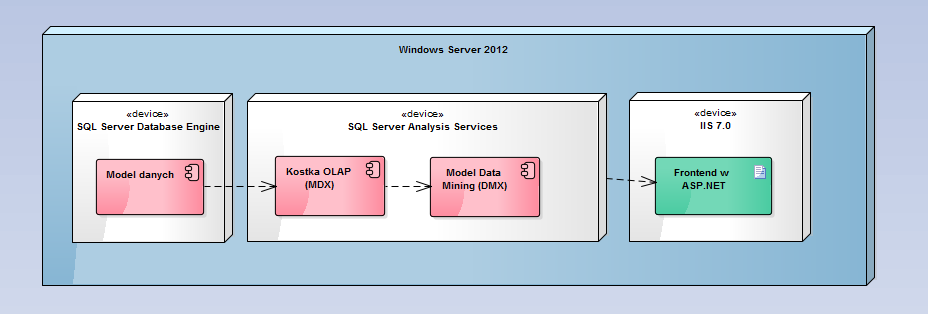
\includegraphics[scale=1]{Architektura.png}\newline
 W architekturze i logice naszego systemu wyróżniamy następujące komponenty:
 \begin{itemize}
 
\item \textbf{Chmura} - Sercem systemu jest główny serwer wraz z innymi usługami znajdujący się w chmurze internetowej. Znajduje się na niej serwer bazy danych, serwer WWW oraz serwer usług analitycznych.

\item \textbf {RDB} - Relacyjna baza danych zawierająca statystyczne dane dotyczące zdawalności przedmiotów przez studentów, ich zapełnienia, popularność itd. Stanowi bazę do tworzenia kostek analitycznych. 

\item \textbf {Kostka OLAP} - struktura danych, która pozwala na szybką analizę danych. Przechowuje ona dane w sposób bardziej przypominający wielowymiarowe arkusze kalkulacyjne niż tradycyjną, relacyjną bazę danych. Rozmieszczenie danych w kostkach pokonuje ograniczenia relacyjnych baz danych.

\item \textbf{Analysis Service} - usługi analityczne dokonujące analizy danych za pomocą algorytmów uczenia maszynowego oraz data mining.
 
\item \textbf{USOS Api} - API udostępniane przez system USOS. Nasz system wykorzystuje je w celu zebrania danych zalogowanego użytkownika niezbędnych do zarekomendowania mu tego czego oczekuje.

\item \textbf{Strona WWW} - interfejs za pomocą którego użytkownik może przesyłać prośby o wykonanie udostępnianych przez system rekomendacji.

\item \textbf{Serwer WWW} - udostępnia użytkownikom stronę internetową, w naszym systemie pośredniczy między interfejsem użytkownika a bazą danych.
  
\end{itemize}

\newpage

Schemat działania i komunikacji między poszczególnymi komponentami wygląda następująco:
\begin{enumerate}

\item Na samym początku działania system tworzy relacyjną bazę danych zawierającą dane statystyczne z USOSa. 

\item Po stworzeniu bazy danych system wykorzystuje usługi Analysis Services w celu stworzenia kostki analitycznej.

\item Po utworzeniu kostki system wykorzystuje usługi Analisys Services w celu przeprowadzenia analizy
danych na kostce i utworzenia odpowiednich modeli predykcyjnych.

\item Po udanym stworzeniu modeli aktywuje się serwer WWW i system staje się dostępny dla użytkowników. 

\item Użytkownik wchodzi na stronę i wysyła żądanie na serwer WWW.

\item Serwer WWW generuje stronę z formularzem zalogowania się.

\item Po odebraniu danych logowania, w przypadku sukcesu, serwer pobiera dane użytkownika przez USOS Api i zwraca stronę WWW - interfejs użytkownika.

\item Serwer WWW po odebraniu prośby o rekomendacje przesyła żądanie do serwera bazy danych o dokonanie predykcji wykorzystując odebrane wcześniej dane użytkownika.

\item Serwer WWW odbiera rezultat zapytania i wyświetla go użytkownikowi.

\end{enumerate}



 \chapter{Technologia}
Technologie wykorzystywane w naszym systemie: \par

 \begin{minipage}{\linewidth}
            \centering
            \includegraphics[width=10cm, height = 3cm]{Azure.jpg}
\end{minipage} \\ \\
\noindent 
 \textbf{Microsoft Azure} - Azure jest komercyjną platformą obsługiwaną przez Microsoft. Udostępnia ona usługi związane z chmurą internetową (tzw cloud-computing). W naszym systemie znajduje sie na niej serwer WWW a także serwer bazy danych. \par ~\\
\begin{minipage}{\linewidth}
            \centering
            
\includegraphics[width=10cm, height = 3cm]{sql-server-2014-logo.png}
\end{minipage} \\ \\

\noindent \textbf{Microsoft SQL Server 2014} - Komercyjny serwer bazodanowy udostępniany przez Microsoft. Znajduje się w nim relacyjna baza danych zawierająca dane niezbędne do stworzenia modelu analitycznego.  \par ~\\

\begin{minipage}{\linewidth}
            \centering
            
\includegraphics[width=4cm, height = 4cm]{R.png}
\end{minipage} \\ \\

\textbf{R} - język skryptowy używany w celu analizy danych a także obliczania predykcji dla studentów bądź uniwersytetu. \par
\begin{itemize}

\begin{figure}
\centering
\begin{minipage}{0.45\textwidth}
\centering

\includegraphics[width=6cm, height = 3cm]{python-logo-master-v3-TM.png}
\end{minipage}\hfill
\begin{minipage}{0.45\textwidth}
\centering

\includegraphics[width=6cm, height = 3cm]{django-logo-negative.png}
\end{minipage}
\end{figure}

\item \textbf{Python oraz Django} - technologie, za pomocą których tworzymy webowy interfejs użytkownika. \par ~\\

\begin{minipage}{\linewidth}
            \centering
            
\includegraphics[width=7cm, height = 2.5cm]{usosapi.jpg}
\end{minipage} \\ \\

\item \textbf {USOS Api} - API udostępniane przez system USOS. Nasz system wykorzystuje go w celu zebrania danych zalogowanego użytkownika
niezbędnych do rekomendacji.

\end{itemize}

\chapter{Funkcjonalności}

Przy wejciu na stronę systemu użytkownik zostaje poproszony o wybranie opcji logowania : "Logowanie dla Studentów" bądź "Logowanie dla Pracowników". Poniższe podrozdziały opisują funkcjonalności zależne od wybranej opcji.

\section{Funkcjonalności dla Studentów}

W tym podrozdziale znajduje się opis funkcjonalności dostępnych dla użytkownika po wybraniu przy logowaniu do systemu opcji "Logowanie dla Studentów".

\subsection{Predykcja ocen}

Student wybiera w systemie opcję predykcji ocen. Następnie wybiera z odpowiedniego menu przedmiot z którego oczekuje predykcji. System na podstawie danych studenta pobranych za pomocą USOS API przy logowaniu dokonuje odpowiedniej predykcji i zwraca ją studentowi w widocznym polu zatytułowanym "Przewidywana ocena".

\subsection{Remomendacja seminariów}

Po wybraniu opcji rekomendacji seminariów student staje przed wyborem dwóch opcji : wybierz najlepsze bądź pokaż ranking. W obu wypadkach system korzysta z pobranego za pomocą USOSApi programu studiów studenta. Jeżeli student ma więcej niż 1 aktywny kierunek studiow, system prosi go o wybór programu, dla którego predykcja seminariów go interesuje. W zależności od wybranej opcji student otrzymuje jedno seminarium które wg systemu najbardziej pasuje do studenta badź też ranking seminariów od najbardziej pasującego do najmniej wg predykcji systemu.

\subsection{Rekomendacja przedmiotów}
Po wybraniu opcji rekomendacji przedmiotów student otrzymuje wybór kilku opcji. Może wybrać opcje "dobierz przedmioty do seminarium", "dobierz przedmioty do zainteresowań" bądź "znajdź najłatwiejsze". W przypadku wyboru pierwszej z nich, student jest proszony o wybór interesującego go seminarium. Na tej podstawie system zwraca listę 5 przedmiotów których student nie zdawał, które są wg systemu najbardziej powiązane z wybranym seminarium. W przypadku wyboru drugiej opcji, student otrzymuje listę 5 przedmiotów powiązanych z jego programem studiów, które najbardziej do niego pasują na podstawie zaliczanych przez niego przedmiotów i wyników z nich otrzymanych. W przypadku wyboru trzeciej opcji, system zwraca 5 przedmiotów powiązanych z programem studiów, które według predykcji student ma największą szansę zdać na dobrą ocenę.

\section{Funkcjonalności dla Administracji}

Poniższy podrozdział opisuje funkcjonalność dostępną po zalogowaniu przez opcję "Logowanie dla Pracowników".

\subsection{Predykcja popularności przedmiotów}
Po wybraniu opcji przewidywania popularności przedmiotów pracownik z menu może wybrać przedmiot, a następnie osobę prowadzącą i semestr akademicki. Na podstawie tych danych system zwraca przewidywaną liczbę osób zapisanych na przedmiot w polu zatytułowanym "przewidywana liczba uczestników".

\begin{thebibliography}{99}
\addcontentsline{toc}{chapter}{Bibliografia}
\bibitem[MDX]{MDX} 	
\emph{Professional Microsoft SQL Server 2012 Analysis Services with MDX and DAX},
Sivakumar Harinath, Ronald Pihlgren, Denny Guang-Yeu Lee, John Sirmon, Robert M. Bruckner,
October 2012
\bibitem[SSAS]{SSAS} 
\emph{Expert Cube Development with SSAS Multidimensional Models},
Chris Webb, Alberto Ferrari, Marco Russo,
February 2014
\bibitem[SQL2014]{SQL2014} 
\emph{Professional Microsoft SQL Server 2014 Integration Services},
Brian Knight, Devin Knight, Jessica M. Moss, Mike Davis, Chris Rock,
June 2014
\bibitem[technet]{technet}
http://technet.microsoft.com/en-us/sqlserver/cc510300.aspx
\bibitem[ASP.NET]{ASP.NET}
http://www.asp.net/mvc
\end{thebibliography}
\end{document}